\documentclass[../dissertation.tex]{subfiles}
\begin{appendices}

\chapter{Additional Information}

\section{MoSCoW Requirements}
\label{sec:moscow}

After defining the scope of the project in Section \ref{sec:scope}, the below MoSCoW requirements \cite{moscowreq} were made. 

Must Have:
\begin{itemize}
    \item A web endpoint that calls the Tulip Python API
	\item To be able to deal with large data (that is too large to just send of the network and be visualised be the client without manipulation)
	\item A basic demo interface
	\item To have data that can be rendered returned from the endpoint
\end{itemize}

Should Have:
\begin{itemize}
    \item A neat JavaScript client, with neat meaning a well-documented list of functions that the client can call that then make calls to the web end-point
	\item A flexible web endpoint, with flexible meaning covers as many relevant API calls as possible, and making sure that as few of the parameters for the API calls are hard-coded. This has the benefit of both:
	\begin{itemize}
	    \item Making the system more useful for a larger number of clients
        \item Letting users make more than just a JavaScript client, so if they want to make a C\# or Java app that would not be a problem
	\end{itemize}
\end{itemize}
	
Could Have:
\begin{itemize}
    \item The ability to ask for an image to be returned if client is low power: This would mean that the visualisation would not be interactive, but would take very little time to transfer the image and next to no time to render it, as opposed to far more time for both tasks to send a network to be constructed on the client.
	\item The ability for a user to link their hosted data to the application: This could be an in-house solution such as a a company network storage, or an external data host such as Amazon's S3 \cite{amazons3}. Hence, big data (hundreds of gigabytes or terrabytes) could be linked to the system with ease, each one being imported and linked to the system manually, or an XML/JSON file could be provided that allowed for batch uploading of data. 
\end{itemize}
	
Won't have but would like:
\begin{itemize}
    \item A fully fledged and pretty interface: It would be nice to have a fully completed front-end that is very user-friendly and has been thoroughly evaluated and tested. However, given the amount of time available for the project, it was decided that this is not as critical as having back-end functionality, and additionally that the front-end is being created to demonstrate what the back-end can do as much as to be part of the project.
\end{itemize}

\section{Technical Infrastructure Sketch}
\label{sec:tech_infra_app}

See Figure \ref{fig:techinfra_app} for first draft of the technical infrastructure.

\begin{figure}
    \centering
    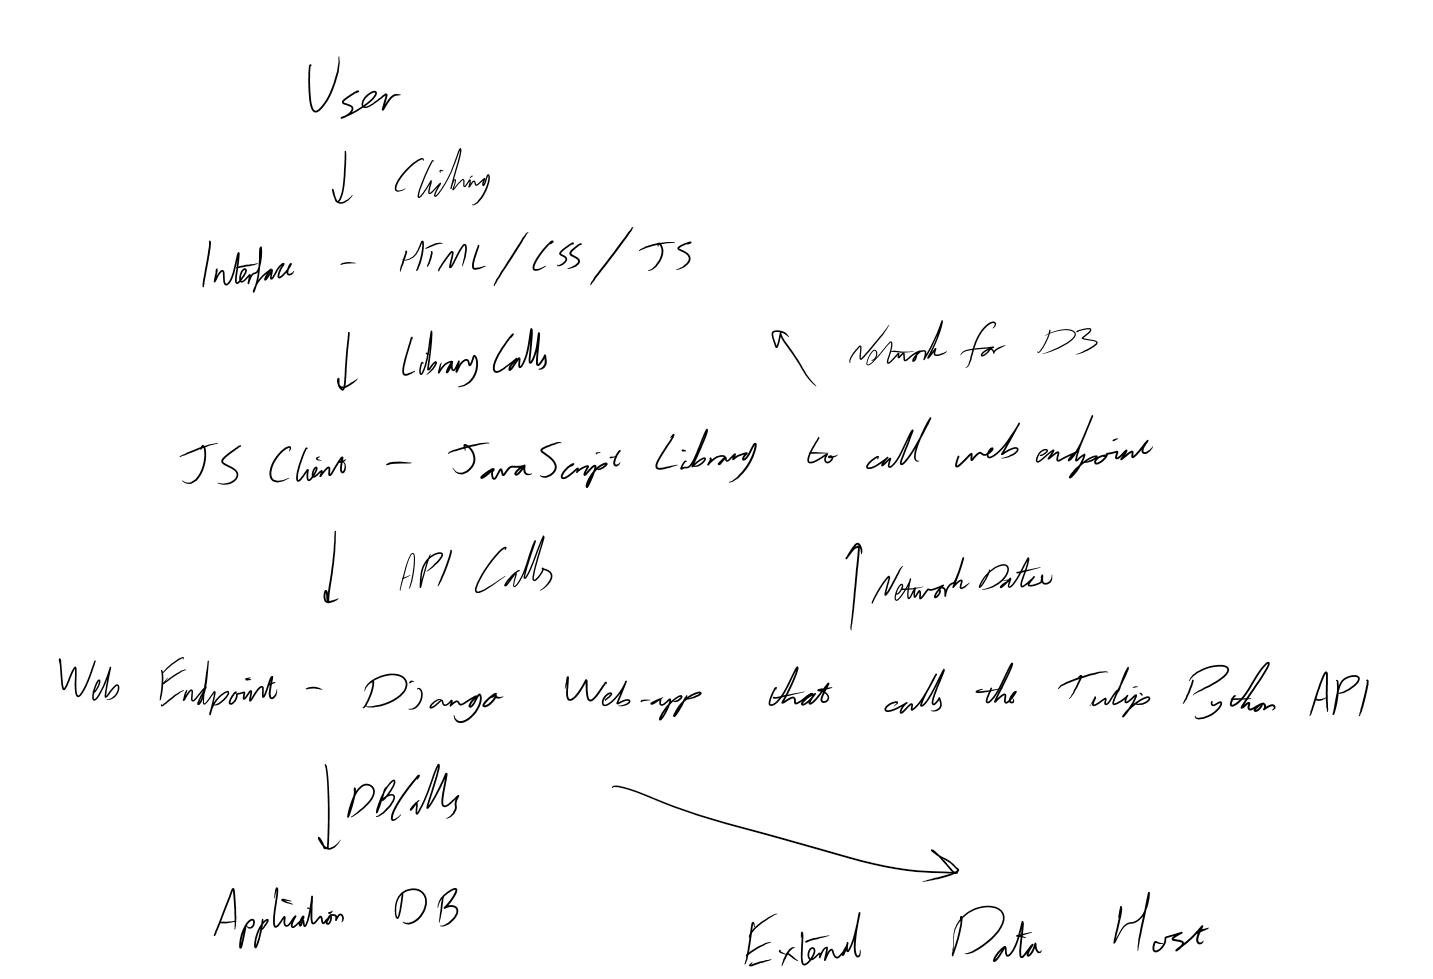
\includegraphics[width=17cm]{6/tech_infra}
    \caption{Draft of Technical Infrastructure}
    \label{fig:techinfra_app}
\end{figure}

\section{What is Hadoop?}
\label{sec:whatishadoop}

Hadoop is a set of open source programs that contain four core modules. These are:

\begin{itemize}
    \item Hadoop Common: The common utilities that support the other Hadoop modules.
    \item Hadoop Distributed File System (HDFS™): A distributed file system that provides high-throughput access to application data.
    \item Hadoop MapReduce: A YARN-based system for parallel processing of large data sets.
    \item Hadoop YARN: A framework for job scheduling and cluster resource management.
\end{itemize}

These combine to give a way of storing, scheduling and processing Big Data in parallel. The way Hadoop could be utilised by the developed application is by storing all of the data that is to be visualised on HDFS, using YARN to schedule the node and edge bundling jobs and the manage the resources available to the cluster where the jobs would be run, and then using MapReduce to process each of the sub-networks then combine them back in to one network.



%----------------------------------

\chapter{Using the Software}

\section{Running the Server}

How to run everything.

\section{Using the Interface}

How to run everything.

% Should I have API calls?

\end{appendices}
